\documentclass[tikz,border=2mm]{standalone}
\definecolor{structure}{HTML}{1A535C}
\definecolor{main}{HTML}{C6892A}
\definecolor{third}{HTML}{8B2635}

\begin{document}

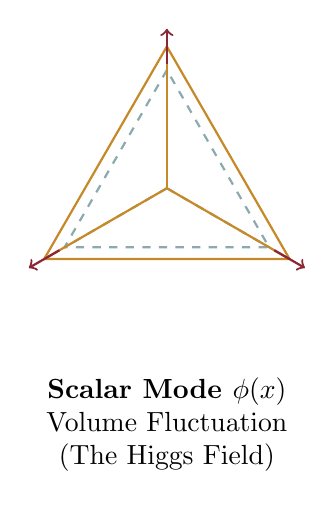
\begin{tikzpicture}[scale=1.5]

% Unperturbed simplex (dashed, original volume)
\draw[thick, structure!50, dashed] (90:1)  -- (210:1) -- (330:1) -- cycle;
\draw[thick, structure!50, dashed] (0,0) -- (90:1);
\draw[thick, structure!50, dashed] (0,0) -- (210:1);
\draw[thick, structure!50, dashed] (0,0) -- (330:1);

% Perturbed simplex (solid, expanded volume)
\draw[thick, main] (90:1.2)  -- (210:1.2) -- (330:1.2) -- cycle;
\draw[thick, main] (0,0) -- (90:1.2);
\draw[thick, main] (0,0) -- (210:1.2);
\draw[thick, main] (0,0) -- (330:1.2);

% Breathing arrows (outward expansion)
\foreach \angle in {90, 210, 330} {
    \draw[->, third, thick] (\angle:1.05) -- (\angle:1.35);
}

% Annotation
\node[align=center] at (0, -2)
    {\textbf{Scalar Mode $\phi(x)$} \\ Volume Fluctuation \\
     (The Higgs Field)};

\end{tikzpicture}

\end{document}
